\documentclass[11pt]{report}

\usepackage[a4paper,margin=1in]{geometry}
\usepackage[T1]{fontenc}
\usepackage[utf8]{inputenc}
\usepackage{lmodern}
\usepackage{amsmath}
\usepackage{booktabs}
\usepackage{array}
\usepackage{tabularx}
\usepackage{longtable}
\usepackage{siunitx}
\usepackage{xcolor}
\usepackage{hyperref}
\usepackage{caption}
\usepackage{graphicx}
\usepackage{tikz}
\usepackage{pgfplots}
\usepackage{pgfplotstable}

\usetikzlibrary{arrows.meta,positioning,shapes.geometric}
\pgfplotsset{compat=1.18}
\sisetup{detect-all,round-mode=places,round-precision=2}

\definecolor{earthgreen}{HTML}{2F6B52}
\definecolor{earthgold}{HTML}{D59B42}
\definecolor{earthblue}{HTML}{2E5EAA}
\definecolor{earthred}{HTML}{B34D3E}
\definecolor{earthteal}{HTML}{2F8F9D}
\definecolor{eartholive}{HTML}{7A8F3D}
\definecolor{softgrid}{HTML}{D9E1E5}

\definecolor{resnet18scratch}{HTML}{3B7EA1}
\definecolor{resnet18pre}{HTML}{58A4B0}
\definecolor{resnet50scratch}{HTML}{B85C38}
\definecolor{resnet50pre}{HTML}{D99962}
\definecolor{vitscratch}{HTML}{556B2F}
\definecolor{vitpre}{HTML}{95B46A}

\hypersetup{
    colorlinks=true,
    linkcolor=earthblue,
    citecolor=earthgreen,
    urlcolor=earthblue
}

\newcommand{\ProjectTitle}{EuroSAT Land-Use Classification with CNNs and Vision Transformers}
\newcommand{\AuthorName}{Jesse Levine}
\newcommand{\StudentID}{101185127}
\newcommand{\CourseName}{SYSC 5108}

\newcommand{\BestModel}{ResNet50 with ImageNet pretraining}
\newcommand{\BestAcc}{98.67}
\newcommand{\BestMacroFOne}{98.62}
\newcommand{\BestLoss}{0.0458}
\newcommand{\EuroSATPaperAcc}{98.57}

\begin{document}
\pagenumbering{gobble}

\begin{titlepage}
    \centering
    \vspace*{4.3cm}
    {\Huge\bfseries \ProjectTitle\par}
    \vspace{0.35cm}
    {\Large\itshape \CourseName\par}
    \vspace{2.2cm}
    {\Large \AuthorName\ (\StudentID)\par}
\end{titlepage}

\pagenumbering{roman}

\chapter*{Abstract}
\addcontentsline{toc}{chapter}{Abstract}
This project studies satellite land-use classification on the EuroSAT RGB dataset using three image classifiers: ResNet18, ResNet50, and ViT-Small. Each backbone was trained both from scratch and from ImageNet-pretrained weights under the same deterministic \(70/15/15\) train/validation/test split. The experiments focus on three questions: how CNNs compare with a vision transformer on a modest remote-sensing dataset, how much transfer learning helps, and how model size relates to accuracy and runtime. The saved results show a clear and consistent effect from pretraining. \BestModel{} was the strongest configuration, reaching \BestAcc{}\% test accuracy, \BestMacroFOne{}\% macro F1, and a test loss of \BestLoss. The pretrained ViT-Small was close behind at \(98.54\%\) test accuracy, while the from-scratch ViT-Small was the weakest run at \(90.40\%\). Overall, the experiments indicate that transfer learning is the dominant factor in this project, and that a pretrained CNN remains the most reliable option for this EuroSAT setting.

\chapter*{Table of Acronyms}
\addcontentsline{toc}{chapter}{Table of Acronyms}
\begin{tabularx}{\textwidth}{>{\bfseries}l X}
    CNN & Convolutional Neural Network \\
    RGB & Red, Green, Blue image channels \\
    GPU & Graphics Processing Unit \\
    ViT & Vision Transformer \\
    F1 & Harmonic mean of precision and recall \\
\end{tabularx}

\chapter*{Table of Math Notations}
\addcontentsline{toc}{chapter}{Table of Math Notations}
\begin{tabularx}{\textwidth}{>{\bfseries}l X}
    \(x\) & Input RGB satellite image patch. \\
    \(y\) & Ground-truth land-use label. \\
    \(\hat{y}\) & Predicted class-probability vector. \\
    \(f_{\theta}(x)\) & Model with parameters \(\theta\). \\
    \(\mathcal{L}_{\mathrm{CE}}\) & Cross-entropy loss used for training. \\
\end{tabularx}

\tableofcontents
\clearpage
\pagenumbering{arabic}

\chapter{Introduction}
Satellite imagery is a practical source of information for land-use mapping, agricultural monitoring, environmental assessment, and urban planning. In agriculture, land-use maps help distinguish cropland, pasture, permanent crops, and surrounding vegetation, which supports crop monitoring, irrigation planning, and broader estimates of land productivity. In urban planning, the ability to separate residential, industrial, transportation, and water-adjacent areas helps planners monitor urban growth, road-network expansion, and the interaction between built and natural environments. Environmental assessment also depends on this type of classification, since changes in vegetation cover, water bodies, and human development can indicate ecosystem stress, habitat change, or unsustainable land conversion.

These applications benefit from automated classification because manual inspection does not scale to modern satellite archives. A human analyst can interpret small samples accurately, but reviewing tens of thousands of image patches is slow, expensive, and difficult to repeat consistently. An automated system with roughly \(98\%\) accuracy changes the workflow substantially: instead of spending most effort on routine labeling, analysts can use the model to process large regions quickly and then focus their attention on ambiguous or high-stakes cases. In practice, this means faster map updates, lower annotation effort, and a much more realistic path toward region-wide monitoring than fully manual interpretation.

Deep learning is a natural candidate for this problem because it can learn discriminative spatial features directly from image patches instead of depending on handcrafted descriptors. Earlier computer-vision approaches often relied on manually designed features such as SIFT, HOG, texture histograms, or color statistics. Those descriptors can work well for constrained object-recognition tasks, but remote-sensing imagery is challenging in ways that make handcrafted pipelines less reliable. Land-use classes may differ by subtle texture, repeated spatial arrangement, and scene context rather than by a single dominant object. The same class can also appear quite different across seasons, illumination conditions, and local geography, while different classes may look deceptively similar in small patches. Handcrafted features are usually too rigid to capture all of these variations well.

By contrast, deep neural networks learn hierarchical representations from data. Early layers can capture edges and local textures, while deeper layers combine those cues into higher-level spatial patterns that are more useful for separating classes such as \textit{PermanentCrop}, \textit{HerbaceousVegetation}, \textit{Residential}, and \textit{Industrial}. This ability to adapt the feature representation to the dataset is a major reason deep learning has become the dominant approach for image classification, including remote sensing. It is also why this project compares two major deep-learning families, convolutional residual networks and vision transformers, rather than relying on a classical feature-engineering pipeline.

This report focuses on the EuroSAT RGB dataset, a balanced benchmark of \(27{,}000\) Sentinel-2 image patches across ten land-use classes \cite{helber2019}. The project investigates three related questions. First, how do CNN baselines compare against a vision transformer on the same task? Second, how much does transfer learning improve performance? Third, is a larger model always worth its extra compute cost on this dataset?

The objective is not to claim a new state of the art, but to produce a clear end-to-end experimental study with reproducible training, validation, and test results. The final outcome is a compact comparison across six runs together with conclusions about convergence speed, class-level behavior, and the effect of transfer learning.

\chapter{Background}
\section{Remote-Sensing Image Classification}
EuroSAT was introduced as a benchmark for land-use and land-cover classification using Sentinel-2 imagery \cite{helber2019}. The dataset provides ten balanced classes and reports strong CNN baselines, including an overall accuracy of \(98.57\%\) in the original paper. That published number gives a useful reference point for this course project, although the split protocol and implementation details differ, so only broad comparisons are appropriate.

Beyond the original EuroSAT baselines, remote-sensing image classification has been studied with several other standard deep architectures. VGG-style networks \cite{simonyan2015} are a common reference because they represent the classic deep CNN approach of stacking many convolutional layers in a simple sequential pattern. DenseNet models \cite{huang2017} are also frequently discussed in image-classification literature because they promote feature reuse by concatenating outputs from earlier layers into later ones, which can improve efficiency and gradient propagation. Together with residual networks and more recent transformer-based models, these architectures form the broader design space that motivates the model choices in this project.

\section{Selected Deep Learning Techniques}
\noindent This section introduces the main deep learning ideas used in this project: residual convolutional networks, vision transformers, and transfer learning.

\subsection{Residual Networks}
Residual networks were introduced to address a specific optimization problem that appeared when CNNs became deeper \cite{he2016}. Earlier ``plain'' CNNs typically stacked convolution, nonlinearity, and pooling layers sequentially, with each layer expected to learn a complete transformation of its input. In principle, adding more layers should increase representational power, but in practice very deep plain networks often showed a degradation effect: training error increased as depth increased, even when overfitting should have made the deeper model at least as good as a shallower one. This indicated that the problem was not only lack of capacity, but also difficulty in optimization.

The key idea in a residual network is to replace direct layer-wise mapping with residual learning. Instead of asking a block to learn a full mapping \(H(x)\), ResNet reformulates the problem as learning a residual function \(F(x) = H(x) - x\), so that the block output becomes
\[
y = F(x) + x.
\]
The added identity path is implemented with a skip connection that bypasses one or more convolutional layers. If the residual function is near zero, the block can simply preserve the input, which makes very deep models easier to train. In effect, the optimizer no longer needs to relearn identity mappings through many stacked nonlinear layers; it only has to learn what should change relative to the input.

This design differentiates residual networks from classic CNNs in several practical ways. First, the skip connection improves gradient flow during backpropagation, reducing the vanishing or weakening of useful training signals across depth. Second, residual blocks make it safer to scale a model upward, because extra layers are less likely to damage performance purely through optimization difficulty. Third, ResNets still retain the core inductive biases of CNNs, namely local receptive fields, weight sharing, and translation-aware feature extraction. That makes them especially suitable for visual problems where nearby pixels form meaningful textures and edges, including satellite imagery.

In this project, ResNet18 serves as the lightweight CNN baseline and ResNet50 as the higher-capacity CNN. Comparing them is useful because they share the same residual-network design philosophy but differ substantially in depth and representational capacity. ResNet18 uses simpler basic residual blocks and is easier to optimize, while ResNet50 uses deeper bottleneck blocks that can model richer feature hierarchies but usually benefit more from transfer learning.

\subsection{Vision Transformers}
\subsubsection{Attention}
Before introducing Vision Transformers, it is useful to explain attention itself. In a neural-network context, attention is a mechanism that allows the model to assign different importance weights to different parts of its input when forming an internal representation or prediction. Instead of treating every token or spatial region equally, the model can learn to focus more strongly on the elements that are most relevant to the current decision. In sequence modeling, this idea became especially influential through the transformer architecture \cite{vaswani2017}. In vision, the same idea can be applied to image regions or patches.

The defining transformer variant is self-attention \cite{vaswani2017}. In self-attention, each input token is compared with every other token in the same sequence. For each token, the model computes query, key, and value projections, then uses similarity between queries and keys to produce attention weights that determine how much information should be gathered from the values of other tokens. This allows each token representation to be updated using context from the entire input rather than only from a fixed local neighborhood.

\subsubsection{Vision Transformers}
Vision Transformers approach image classification from this attention-based perspective rather than from convolution. They adapt the transformer architecture originally developed for sequence modeling and machine translation \cite{vaswani2017} to visual inputs \cite{dosovitskiy2021}. Instead of processing an image with sliding convolutional kernels, a ViT divides the image into fixed-size patches, linearly embeds each patch into a token vector, adds positional information, and then feeds the token sequence into stacked self-attention layers. A special class token aggregates information for the final prediction.

This allows information from distant spatial regions to be mixed directly in a single layer, whereas a CNN usually builds long-range context gradually across many convolutional stages. Because of this, transformers are often described as having more global and more flexible feature interactions than classic CNNs.

At the same time, ViTs do not encode the same built-in visual assumptions as CNNs. A convolutional layer already assumes that nearby pixels are related and that the same local patterns may appear anywhere in the image. A transformer is more generic: it can learn those patterns, but it is not forced to start with them. This weaker inductive bias is part of what makes ViTs powerful at scale, but it also helps explain why they are often less data-efficient than CNNs when trained from scratch on smaller datasets. For a dataset such as EuroSAT, this trade-off is important because the benchmark is large enough to support meaningful training, but still far smaller than the image collections typically used to train transformers from scratch successfully.

ViT-Small is therefore an informative comparison point in this project. It represents a modern non-convolutional vision backbone with a parameter count similar to ResNet50, but it processes spatial structure in a fundamentally different way. Including it makes it possible to compare not only small versus large models, but also convolutional versus attention-based representations under the same dataset split and optimization pipeline.

\subsection{Transfer Learning}
Transfer learning refers to the practice of taking knowledge learned on one task or dataset and reusing it to improve performance on a different but related task \cite{pan2010}. In deep learning for vision, the most common form is to start from a model that has already been trained on a large benchmark such as ImageNet \cite{deng2009}, then adapt that model to a smaller target dataset by replacing or fine-tuning the final classifier layers. This is attractive because the pretrained network has already learned many useful low-level and mid-level visual features, such as edges, textures, color transitions, shape fragments, and other recurring image patterns.

For a dataset such as EuroSAT, transfer learning is especially important because the dataset is meaningful in size but still much smaller than the image collections typically used to train modern backbones from scratch. A randomly initialized model must learn both general visual primitives and task-specific land-use distinctions from the same limited supervision. By contrast, a pretrained model can begin with a more informative feature space and spend more of its training effort adapting those features to the new domain. In practical terms, this often improves optimization stability, speeds up convergence, and raises final accuracy.

Transfer learning is also relevant for comparing CNNs and transformers fairly. CNNs and transformers have different inductive biases, but both can benefit from initialization on large-scale natural-image data. In this project, all pretrained runs start from ImageNet weights. This makes it possible to study not only how architecture family affects EuroSAT performance, but also how strongly each family depends on prior visual knowledge before fine-tuning on the satellite imagery task.

\section{Architectural Details of the Chosen Models}
The three backbones differ not only in parameter count, but in how they process spatial structure. Both ResNet models begin with a \(7 \times 7\) convolution with stride 2, followed by a \(3 \times 3\) max-pooling layer. After this stem, they stack four residual stages and finish with global average pooling plus a linear classifier adapted to ten EuroSAT classes.

ResNet18 uses the standard \([2,2,2,2]\) stage layout with \texttt{BasicBlock} residual units and a final \(512 \rightarrow 10\) classification head. ResNet50 keeps the same four-stage pattern but expands it to \([3,4,6,3]\) \texttt{Bottleneck} blocks, producing a \(2048 \rightarrow 10\) output layer. This deeper bottleneck design increases representational capacity, but it also raises optimization difficulty when the model is trained from scratch on a relatively small dataset.

The ViT-Small model is instantiated as \texttt{vit\_small\_patch16\_224}. In this project, the EuroSAT images remain \(64 \times 64\), so a patch size of 16 produces only \(4 \times 4 = 16\) image patches. These tokens are projected into a 384-dimensional embedding space, prepended with one class token, and processed by 12 transformer encoder blocks with 6 attention heads and an MLP ratio of 4.0. The final classifier is a \(384 \rightarrow 10\) linear layer. The small number of patches makes the transformer computationally manageable here, but it also means that each token represents a fairly large spatial region of the original image.

\begin{table}[h]
    \centering
    \caption{Concrete architecture details of the three backbones used in code.}
    \begin{tabular}{l l l l}
        \toprule
        Model & Main stem or tokenizer & Core depth & Task-specific head \\
        \midrule
        ResNet18 & \(7 \times 7\) conv + max-pool & \(2,2,2,2\) BasicBlocks & \(512 \rightarrow 10\) \\
        ResNet50 & \(7 \times 7\) conv + max-pool & \(3,4,6,3\) Bottlenecks & \(2048 \rightarrow 10\) \\
        ViT-Small & \(16 \times 16\) patch embedding & 12 transformer blocks, 6 heads & \(384 \rightarrow 10\) \\
        \bottomrule
    \end{tabular}
\end{table}

\section{Why These Models Were Chosen}
The selected models cover two complementary design families and a meaningful range of parameter counts. ResNet18 is small and efficient, ResNet50 is deeper and more expressive, and ViT-Small has a parameter budget similar to ResNet50 while relying on a different inductive bias. This combination makes it possible to separate three effects: architecture family, model capacity, and pretraining.

ResNet was chosen over older plain CNN families such as VGG because it is a stronger and more modern baseline for supervised image classification. VGG is historically important, but its sequential design lacks residual connections and tends to be less parameter-efficient for the level of depth it requires \cite{simonyan2015}. DenseNet is also a credible alternative, and its dense feature reuse can work very well in practice \cite{huang2017}. However, for this project ResNet offered a cleaner baseline because it is widely used, easy to interpret, and available in two well-established scales, ResNet18 and ResNet50, that make capacity comparisons straightforward without changing the overall architectural family.

ViT-Small was chosen to complement the CNN baselines with a fundamentally different style of representation learning. Instead of local convolutions and progressively expanding receptive fields, it uses patch tokens and self-attention to capture global interactions directly. This makes it a useful contrast model for EuroSAT: if ResNet represents a strong conventional vision backbone, ViT represents the modern attention-based alternative. Comparing these two families gives a more meaningful study than comparing several closely related CNN variants, because it tests whether performance differences come from model size alone or from the underlying learning bias of the architecture itself.

\chapter{System Description}
\section{Dataset and Split}
The experiments use the RGB version of EuroSAT with ten classes and \(64 \times 64\) inputs \cite{helber2019}. EuroSAT is derived from Sentinel-2 imagery collected under the Copernicus Earth observation program, and the full dataset contains all 13 Sentinel-2 spectral bands. In this project, only the RGB subset is used, which corresponds to the visible red, green, and blue channels rather than the full multispectral stack. This keeps the task aligned with standard image-classification pipelines while still preserving the remote-sensing context of the original benchmark.

The physical image properties are also important for interpreting the task. Sentinel-2 provides multiple spatial resolutions across its spectral bands, but the RGB channels belong to the \(10\) meter resolution group. As a result, each \(64 \times 64\) RGB patch represents an area of roughly \(640 \times 640\) meters on the ground. This means the classifier is not recognizing individual objects in the way a close-range vision system might; instead, it is learning scene-level land-use patterns such as crop texture, road layout, building density, river structure, and water coverage.

A deterministic stratified split assigns \(70\%\) of the images to training, \(15\%\) to validation, and \(15\%\) to testing. The split is implemented in two stages. First, \(70\%\) of the full dataset is assigned to training and the remaining \(30\%\) is held aside. Second, that held-out portion is split evenly into validation and test subsets. The stratified part means that class labels are used during both split steps so that each subset preserves the same class proportions as the original dataset. Since EuroSAT is class-balanced to begin with, stratification ensures that the final validation and test sets are also balanced rather than accidentally over-representing or under-representing certain classes.

This matters for both fairness and interpretability. If one class were much more common in the test set than another, overall accuracy could be biased toward whatever class distribution happened to appear in that split. By preserving class balance, the \(15\%\) test set contains \(405\) examples from each of the ten classes, for a total of \(4050\) test images. The same logic applies to the validation set, which also contains \(405\) images per class. Because the split is deterministic, the exact same train, validation, and test partitions can be regenerated in later runs, which supports reproducibility across all six model configurations.

\begin{table}[h]
    \centering
    \caption{EuroSAT RGB class distribution under the project split.}
    \begin{tabular}{lrrrr}
        \toprule
        Class & Train & Validation & Test & Total \\
        \midrule
        AnnualCrop & 1890 & 405 & 405 & 2700 \\
        Forest & 1890 & 405 & 405 & 2700 \\
        HerbaceousVegetation & 1890 & 405 & 405 & 2700 \\
        Highway & 1890 & 405 & 405 & 2700 \\
        Industrial & 1890 & 405 & 405 & 2700 \\
        Pasture & 1890 & 405 & 405 & 2700 \\
        PermanentCrop & 1890 & 405 & 405 & 2700 \\
        Residential & 1890 & 405 & 405 & 2700 \\
        River & 1890 & 405 & 405 & 2700 \\
        SeaLake & 1890 & 405 & 405 & 2700 \\
        \midrule
        Total & 18900 & 4050 & 4050 & 27000 \\
        \bottomrule
    \end{tabular}
\end{table}

\section{Preprocessing and Training}
All models use the same image normalization statistics and the same data augmentation policy: random horizontal flips, random vertical flips, and random rotations up to \(180^\circ\). The optimization setup is also fixed across runs: AdamW \cite{loshchilov2019}, a learning rate of \(3 \times 10^{-4}\), weight decay of \(10^{-4}\), a batch size of \(256\), and \(40\) epochs.

This augmentation policy is particularly suitable for satellite imagery because EuroSAT patches are captured from a nadir, or top-down, perspective. Unlike natural photographs, where flipping or rotating an image can create unrealistic object orientations, a farm, forest, river, or residential block can appear in many valid orientations when viewed from above. For that reason, horizontal flips, vertical flips, and \(180^\circ\) rotations help the model learn orientation-robust land-use patterns without violating the physical meaning of the scene.

The learning rate is not kept constant throughout training. Instead, the training script uses cosine annealing, which starts from the initial learning rate and then gradually decreases it over the \(40\) epochs following a cosine-shaped schedule. In practical terms, the updates are larger at the beginning of training, when the model is still making broad adjustments, and smaller near the end, when the model is refining the solution. This is useful because a relatively high early learning rate helps the optimizer move quickly through parameter space, while a lower late learning rate reduces oscillation and makes convergence toward a strong local optimum more stable.

The training and testing process is also designed to separate model fitting from final evaluation. During each epoch, the model is optimized on the training subset and then evaluated on the validation subset without gradient updates. The checkpoint with the highest validation accuracy is saved as the best model, and only that saved checkpoint is run once on the held-out test set. This avoids tuning decisions directly on the test data and makes the reported test accuracy a cleaner estimate of generalization performance.

The training objective is standard multi-class cross-entropy:
\[
\mathcal{L}_{\mathrm{CE}} = -\sum_{c=1}^{C} y_c \log \hat{y}_c.
\]
Model selection is based on the highest validation accuracy, and the corresponding checkpoint is evaluated once on the held-out test set. For all six runs, the final classification layer was replaced so that each backbone predicts the ten EuroSAT classes. This keeps the feature extractor architecture intact while aligning the output space to the project task.

For the pretrained runs, the starting weights come from ImageNet, which contains \(1000\) classes of mostly natural objects and scenes rather than remote-sensing categories. This creates a domain gap between the source task and EuroSAT. However, the lower and intermediate layers of a pretrained model still learn broadly useful visual primitives such as edges, texture transitions, repeated patterns, and color structure. Even though ImageNet does not contain a class called \textit{PermanentCrop}, those general features can still provide a strong starting point for recognizing agricultural and land-use structure after fine-tuning on the satellite dataset.

\begin{table}[h]
    \centering
    \caption{Shared training configuration for all six runs.}
    \begin{tabular}{ll}
        \toprule
        Setting & Value \\
        \midrule
        Dataset & EuroSAT RGB \\
        Input size & \(64 \times 64\) \\
        Train/val/test split & \(70/15/15\) stratified \\
        Epochs & 40 \\
        Batch size & 256 \\
        Optimizer & AdamW \\
        Scheduler & Cosine annealing \\
        Loss function & Cross-entropy \\
        Device & RTX 5080 GPU \\
        Metrics & Accuracy, macro F1, loss, confusion matrix \\
        \bottomrule
    \end{tabular}
\end{table}

\section{System Pipeline}
Figure~\ref{fig:pipeline} summarizes the full workflow used in the project, but the sequence is straightforward. The process begins with the EuroSAT RGB image patches and the deterministic split manifest that assigns each image to the training, validation, or test subset. The training subset is then passed through the augmentation and normalization pipeline, while the validation and test subsets use only resizing and normalization so that evaluation reflects the saved images more directly.

After preprocessing, one of the three backbones, ResNet18, ResNet50, or ViT-Small, is instantiated and trained for up to \(40\) epochs under the shared optimization settings described above. During training, the model parameters are updated only on the training batches, and validation accuracy is measured after each epoch. Whenever validation accuracy improves, the corresponding checkpoint is saved as the current best model. This ensures that the final reported model is selected using validation performance rather than the last epoch by default.

The final stage of the pipeline is evaluation and analysis. Once training is complete, the best checkpoint is reloaded and evaluated on the held-out test set to produce the final loss, overall accuracy, macro F1 score, classification report, and confusion matrix. For the ViT experiments, the saved checkpoint is also used to generate attention visualizations, which provide a qualitative view of where the model focuses when making correct and incorrect predictions.

\begin{figure}[h]
    \centering
    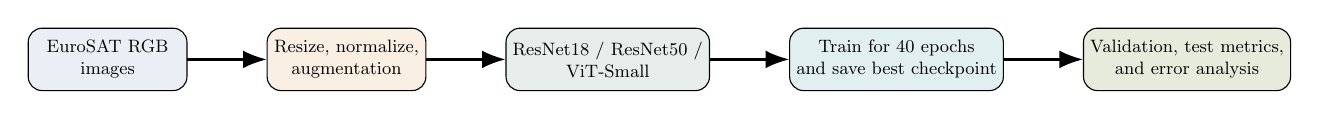
\begin{tikzpicture}[
        scale=0.72,
        transform shape,
        node distance=1.4cm,
        every node/.style={font=\small, align=center},
        stage/.style={draw, rounded corners=5pt, minimum width=2.8cm, minimum height=1.1cm},
        arrow/.style={-{Latex[length=3mm]}, thick}
    ]
        \node[stage, fill=earthblue!10] (dataset) {EuroSAT RGB\\images};
        \node[stage, fill=earthgold!15, right=of dataset] (prep) {Resize, normalize,\\augmentation};
        \node[stage, fill=earthgreen!12, right=of prep] (model) {ResNet18 / ResNet50 /\\ViT-Small};
        \node[stage, fill=earthteal!14, right=of model] (train) {Train for 40 epochs\\and save best checkpoint};
        \node[stage, fill=eartholive!18, right=of train] (eval) {Validation, test metrics,\\and error analysis};
        \draw[arrow] (dataset) -- (prep);
        \draw[arrow] (prep) -- (model);
        \draw[arrow] (model) -- (train);
        \draw[arrow] (train) -- (eval);
    \end{tikzpicture}
    \caption{End-to-end pipeline used in the project.}
    \label{fig:pipeline}
\end{figure}

The pipeline was kept identical across all six runs except for the backbone choice and whether ImageNet pretraining was enabled. Keeping the rest of the process fixed is important because it makes differences in the final results easier to attribute to architecture and initialization rather than to changing data preparation or optimization settings.

\chapter{Numerical Results}
\section{Overall Comparison}
Table~\ref{tab:overall-results} summarizes the six completed training runs. The strongest overall configuration was \BestModel{}, which slightly exceeds the \(98.57\%\) EuroSAT benchmark reported in the dataset paper \cite{helber2019}. That said, the comparison should be interpreted cautiously because the exact split and implementation are not identical.

The small improvement over the published benchmark does not necessarily mean that this project has established a stronger general result than the original paper. A more reasonable interpretation is that several implementation choices in the current pipeline may have been favorable for this specific split. In particular, the best run combines ImageNet pretraining with modern fine-tuning choices such as AdamW optimization, cosine learning-rate decay, and consistent geometric augmentation through flips and rotations. It is plausible that these choices improved convergence and generalization slightly relative to older or different training settings. In addition, the deterministic stratified split used here is not the same evaluation protocol as the one used in the original EuroSAT study, so even a small change in which image patches appear in the test set can shift the final accuracy by a fraction of a percentage point. For that reason, the fairest conclusion is that the pretrained ResNet50 result is broadly consistent with the original EuroSAT benchmark and slightly higher under this project-specific setup, rather than definitively better in a strict apples-to-apples sense.

\begin{table}[h]
    \centering
    \caption{Overall comparison across the six completed runs.}
    \label{tab:overall-results}
    \small
    \begin{tabular}{lrrrrr}
        \toprule
        Run & Params (M) & Test Acc. (\%) & Macro F1 (\%) & Test Loss & Train Time (s) \\
        \midrule
        ResNet18 Scratch & 11.18 & 95.75 & 95.62 & 0.1362 & 34.52 \\
        ResNet18 Pretrained & 11.18 & 98.42 & 98.36 & 0.0516 & 34.65 \\
        ResNet50 Scratch & 23.53 & 93.16 & 92.91 & 0.2202 & 76.02 \\
        ResNet50 Pretrained & 23.53 & 98.67 & 98.62 & 0.0458 & 75.29 \\
        ViT-Small Scratch & 21.60 & 90.40 & 90.08 & 0.3038 & 58.17 \\
        ViT-Small Pretrained & 21.60 & 98.54 & 98.48 & 0.0520 & 57.54 \\
        \bottomrule
    \end{tabular}
\end{table}

Two trends are immediate. First, every pretrained model outperformed its from-scratch counterpart by a large margin. Second, the from-scratch ViT-Small was the least data-efficient model in the study, while the pretrained ViT-Small nearly matched the best CNN.

\section{Training Dynamics}
\begin{figure}[p]
    \centering
    \begin{tikzpicture}
        \begin{axis}[
            width=\textwidth,
            height=0.42\textheight,
            xlabel={Epoch},
            ylabel={Validation accuracy (\%)},
            xmin=1, xmax=40,
            ymin=50, ymax=100,
            grid=both,
            major grid style={softgrid},
            legend style={font=\small, at={(0.5,-0.23)}, anchor=north, legend columns=3},
            tick label style={font=\small},
            label style={font=\small}
        ]
            \addplot[thick, color=resnet18scratch] table[x=epoch, y=val_accuracy_pct, col sep=comma] {data/history_resnet18_eurosat_40ep.csv};
            \addlegendentry{ResNet18 scratch}

            \addplot[thick, color=resnet18pre] table[x=epoch, y=val_accuracy_pct, col sep=comma] {data/history_resnet18_eurosat_40ep_pretrained.csv};
            \addlegendentry{ResNet18 pretrained}

            \addplot[thick, color=resnet50scratch] table[x=epoch, y=val_accuracy_pct, col sep=comma] {data/history_resnet50_eurosat_40ep_bs256.csv};
            \addlegendentry{ResNet50 scratch}

            \addplot[thick, color=resnet50pre] table[x=epoch, y=val_accuracy_pct, col sep=comma] {data/history_resnet50_eurosat_40ep_pretrained_bs256.csv};
            \addlegendentry{ResNet50 pretrained}

            \addplot[thick, color=vitscratch] table[x=epoch, y=val_accuracy_pct, col sep=comma] {data/history_vit_small_eurosat_40ep.csv};
            \addlegendentry{ViT-Small scratch}

            \addplot[thick, color=vitpre] table[x=epoch, y=val_accuracy_pct, col sep=comma] {data/history_vit_small_eurosat_40ep_pretrained.csv};
            \addlegendentry{ViT-Small pretrained}
        \end{axis}
    \end{tikzpicture}
    \caption{Validation accuracy over training epochs for all six runs.}
    \label{fig:val-curves}
\end{figure}

Figure~\ref{fig:val-curves} shows that pretraining changes convergence behavior immediately. The pretrained ResNet50 reached at least \(95\%\) validation accuracy in the first epoch, the pretrained ViT-Small reached it by epoch 3, and the pretrained ResNet18 reached it by epoch 4. In contrast, none of the from-scratch models except ResNet18 ever crossed \(95\%\), and the from-scratch ViT-Small never reached \(90\%\) validation accuracy within 40 epochs.

\section{Accuracy, Capacity, and Transfer Learning}
\begin{figure}[h]
    \centering
    \begin{tikzpicture}
        \begin{axis}[
            width=\textwidth,
            height=0.33\textheight,
            ybar,
            bar width=8pt,
            ymin=88, ymax=100,
            ylabel={Score (\%)},
            symbolic x coords={R18-S,R18-P,R50-S,R50-P,ViT-S,ViT-P},
            xtick=data,
            xticklabels={R18-S,R18-P,R50-S,R50-P,ViT-S,ViT-P},
            xticklabel style={rotate=20, anchor=east},
            legend style={font=\small, at={(0.5,1.02)}, anchor=south, legend columns=2},
            grid=major,
            major grid style={softgrid},
            tick label style={font=\small},
            label style={font=\small}
        ]
            \addplot[fill=earthblue!60, draw=earthblue] coordinates {
                (R18-S,95.75) (R18-P,98.42) (R50-S,93.16) (R50-P,98.67) (ViT-S,90.40) (ViT-P,98.54)
            };
            \addlegendentry{Test accuracy}

            \addplot[fill=earthgold!70, draw=earthgold] coordinates {
                (R18-S,95.62) (R18-P,98.36) (R50-S,92.91) (R50-P,98.62) (ViT-S,90.08) (ViT-P,98.48)
            };
            \addlegendentry{Macro F1}
        \end{axis}
    \end{tikzpicture}
    \caption{Test accuracy and macro F1 for each run. Tick labels use the abbreviations ResNet18 (R18), ResNet50 (R50), and ViT-Small (ViT), with S for scratch and P for pretrained.}
    \label{fig:overall-bars}
\end{figure}

\begin{figure}[h]
    \centering
    \begin{tikzpicture}
        \begin{axis}[
            width=0.9\textwidth,
            height=0.34\textheight,
            xlabel={Parameter count (millions)},
            ylabel={Test accuracy (\%)},
            xmin=10, xmax=24.5,
            ymin=89, ymax=99,
            grid=both,
            major grid style={softgrid},
            legend style={font=\small, at={(0.5,-0.2)}, anchor=north, legend columns=2},
            tick label style={font=\small},
            label style={font=\small}
        ]
            \addplot[only marks, mark=square*, mark size=2.8pt, color=earthblue] coordinates {(11.18,95.75) (23.53,93.16)};
            \addlegendentry{CNN scratch}

            \addplot[only marks, mark=square*, mark size=2.8pt, color=earthgold] coordinates {(11.18,98.42) (23.53,98.67)};
            \addlegendentry{CNN pretrained}

            \addplot[only marks, mark=triangle*, mark size=3pt, color=earthgreen] coordinates {(21.60,90.40)};
            \addlegendentry{ViT scratch}

            \addplot[only marks, mark=triangle*, mark size=3pt, color=earthred] coordinates {(21.60,98.54)};
            \addlegendentry{ViT pretrained}
        \end{axis}
    \end{tikzpicture}
    \caption{Model size versus test accuracy. The figure highlights that pretraining matters more than parameter count alone.}
    \label{fig:params-vs-acc}
\end{figure}

\begin{figure}[h]
    \centering
    \begin{tikzpicture}
        \begin{axis}[
            width=0.82\textwidth,
            height=0.3\textheight,
            ybar,
            bar width=12pt,
            ymin=0, ymax=9,
            ylabel={Accuracy gain (percentage points)},
            symbolic x coords={ResNet18,ResNet50,ViT-Small},
            xtick=data,
            grid=major,
            major grid style={softgrid},
            tick label style={font=\small},
            label style={font=\small}
        ]
            \addplot[fill=earthgreen!60, draw=earthgreen] coordinates {
                (ResNet18,2.67) (ResNet50,5.51) (ViT-Small,8.15)
            };
        \end{axis}
    \end{tikzpicture}
    \caption{Test-accuracy improvement obtained from ImageNet pretraining.}
    \label{fig:pretraining-gain}
\end{figure}

The parameter-count view in Figure~\ref{fig:params-vs-acc} shows that larger models were not automatically better when trained from scratch: ResNet50 scratch was worse than ResNet18 scratch, and ViT-Small scratch was worst overall despite having almost as many parameters as ResNet50. Figure~\ref{fig:pretraining-gain} makes the more important effect explicit. The largest gain from pretraining occurred for ViT-Small, which improved by \(8.15\) percentage points.

\section{Class-Level Behavior}
\begin{table}[h]
    \centering
    \caption{Hardest and easiest classes by per-class F1 score.}
    \label{tab:class-extremes}
    \begin{tabular}{lrrrr}
        \toprule
        Run & Hardest class & F1 (\%) & Easiest class & F1 (\%) \\
        \midrule
        ResNet18 Scratch & PermanentCrop & 91.13 & SeaLake & 99.11 \\
        ResNet18 Pretrained & PermanentCrop & 96.39 & SeaLake & 99.67 \\
        ResNet50 Scratch & PermanentCrop & 86.83 & SeaLake & 99.00 \\
        ResNet50 Pretrained & AnnualCrop & 97.14 & SeaLake & 99.78 \\
        ViT-Small Scratch & Highway & 78.84 & Forest & 96.16 \\
        ViT-Small Pretrained & PermanentCrop & 96.61 & SeaLake & 99.78 \\
        \bottomrule
    \end{tabular}
\end{table}

SeaLake was the easiest class in five of the six runs, while PermanentCrop was usually the hardest. This pattern is plausible because water bodies have strong visual structure, whereas PermanentCrop overlaps with AnnualCrop and HerbaceousVegetation more often.

\begin{figure}[p]
    \centering
    \begin{tikzpicture}
        \begin{axis}[
            width=0.82\textwidth,
            height=0.5\textheight,
            view={0}{90},
            colorbar,
            colormap/viridis,
            xlabel={Predicted class},
            ylabel={True class},
            xmin=0.5, xmax=10.5,
            ymin=0.5, ymax=10.5,
            xtick={1,...,10},
            ytick={1,...,10},
            xticklabels={Annual,Forest,Herbaceous,Highway,Industrial,Pasture,Permanent,Residential,River,SeaLake},
            yticklabels={Annual,Forest,Herbaceous,Highway,Industrial,Pasture,Permanent,Residential,River,SeaLake},
            x tick label style={rotate=45, anchor=east, font=\scriptsize},
            y tick label style={font=\scriptsize},
            y dir=reverse,
            point meta min=0,
            point meta max=405,
            tick label style={font=\small},
            label style={font=\small}
        ]
            \addplot[
                scatter,
                only marks,
                mark=square*,
                mark size=8pt,
                scatter src=explicit,
                point meta=explicit,
                scatter/use mapped color={draw=mapped color, fill=mapped color}
            ] table[x=predicted_index, y=actual_index, meta=count, col sep=comma] {data/confusion_best_model.csv};
        \end{axis}
    \end{tikzpicture}
    \caption{Confusion matrix for the best model, ResNet50 with ImageNet pretraining.}
    \label{fig:confusion}
\end{figure}

The confusion matrix in Figure~\ref{fig:confusion} is strongly diagonal, which matches the near-\(99\%\) accuracy of the best runs. The remaining errors are concentrated in semantically similar classes. For example, the largest off-diagonal counts for the best model include PermanentCrop \(\rightarrow\) AnnualCrop and Pasture \(\rightarrow\) AnnualCrop, each with eight mistakes.

The repeated confusion between PermanentCrop and HerbaceousVegetation suggests a useful direction for improvement. In RGB imagery alone, these classes can share very similar green texture and spatial appearance, especially when the patch does not include strong geometric cues such as field boundaries or surrounding infrastructure. One likely fix would be to use the full multispectral EuroSAT data instead of only RGB, because near-infrared and red-edge information is often more informative for distinguishing vegetation type and crop condition than visible color alone. A second improvement would be to incorporate more spatial context, for example by training on larger image crops or using a multi-scale pipeline, since the arrangement of fields and nearby land cover may help separate permanent agricultural patterns from more generic herbaceous vegetation. Finally, this class pair could benefit from targeted error-aware augmentation or class-focused fine-tuning so that the model sees more hard borderline examples during training.

\section{Attention-Map Batch Summary}
The project also saved a small batch of ViT-Small attention visualizations. Since these figures already exist as report-ready raster outputs, it is more useful to show representative examples directly. Figure~\ref{fig:attention-montage} includes two correct and two incorrect cases from the saved batch.

\begin{figure}[p]
    \centering
    \begin{minipage}[t]{0.48\textwidth}
        \centering
        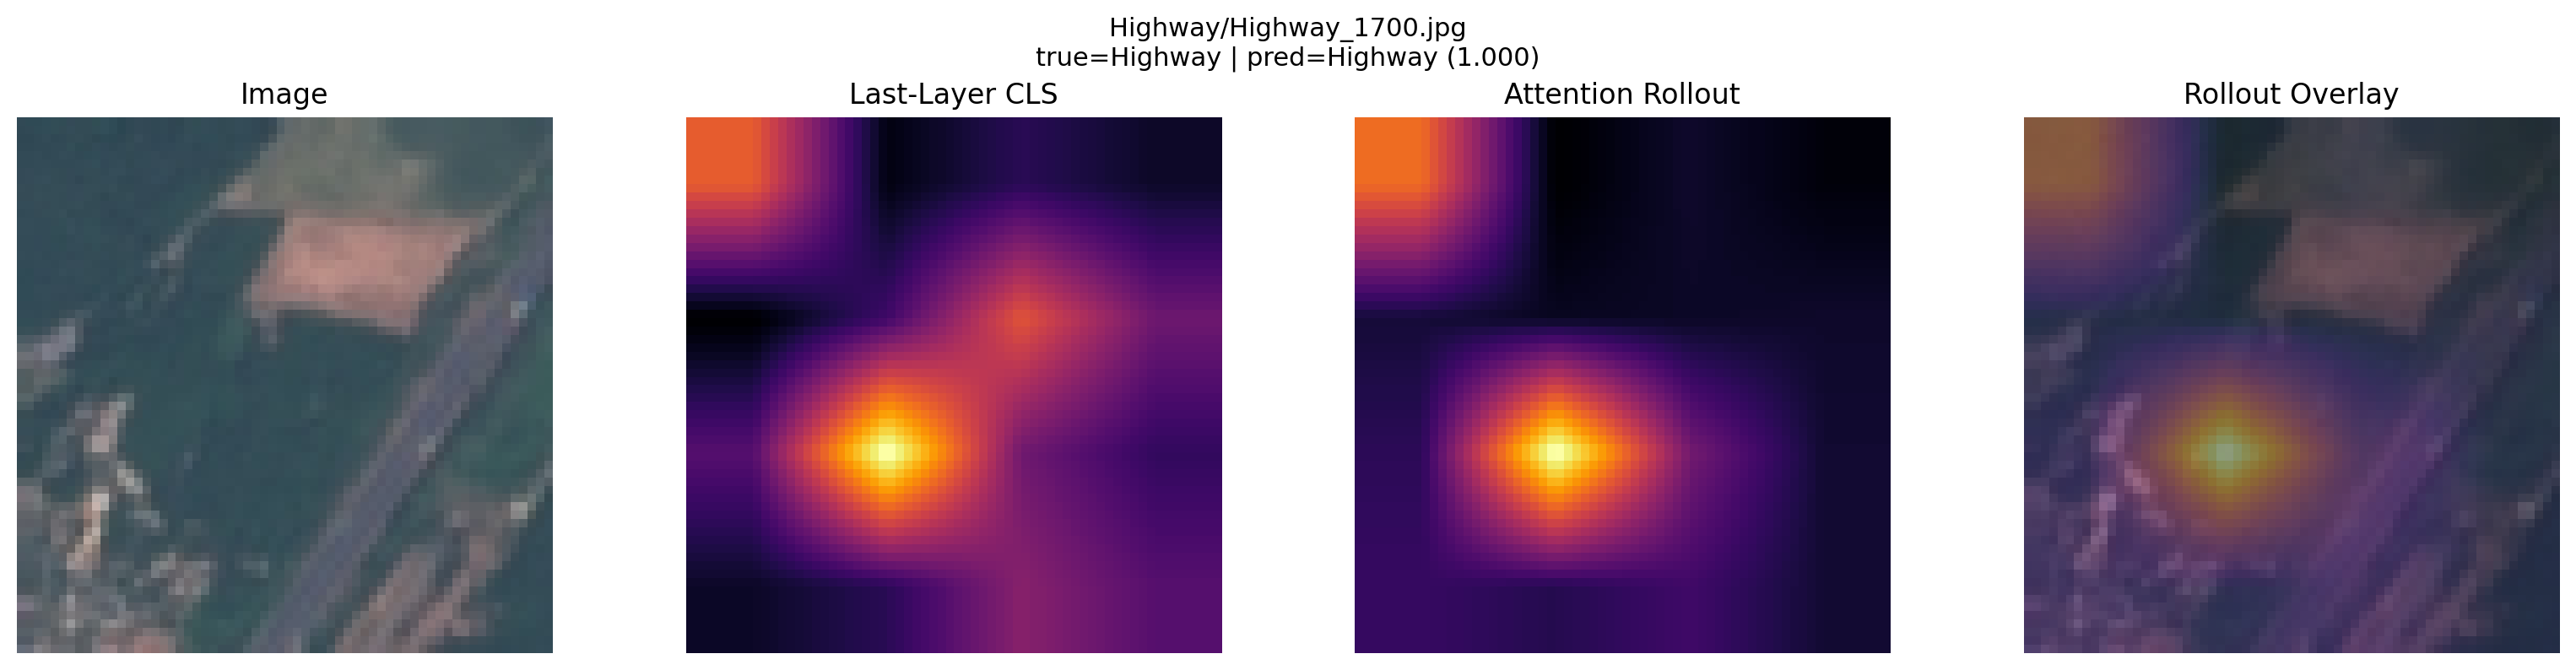
\includegraphics[width=\linewidth]{../outputs/vit_attention_batch/Highway_1700_correct_attention.png}
        \caption*{\footnotesize Correct: Highway \(\rightarrow\) Highway (99.998\%)}
    \end{minipage}
    \hfill
    \begin{minipage}[t]{0.48\textwidth}
        \centering
        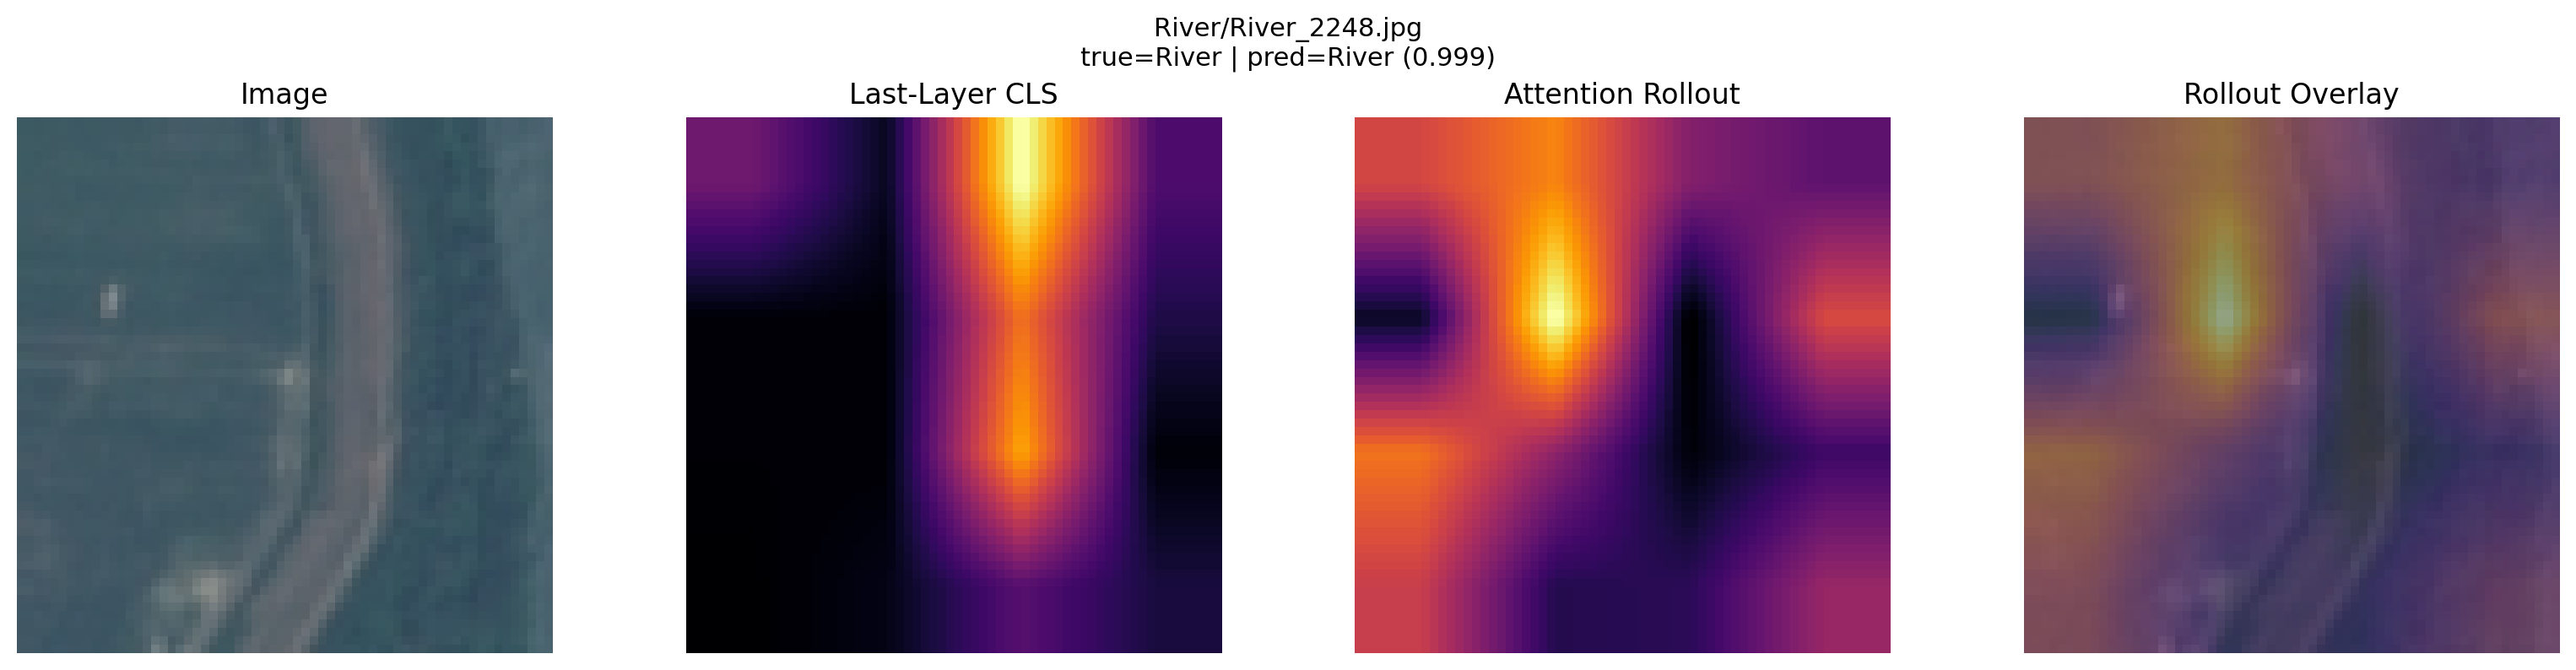
\includegraphics[width=\linewidth]{../outputs/vit_attention_batch/River_2248_correct_attention.png}
        \caption*{\footnotesize Correct: River \(\rightarrow\) River (99.95\%)}
    \end{minipage}

    \vspace{0.9em}

    \begin{minipage}[t]{0.48\textwidth}
        \centering
        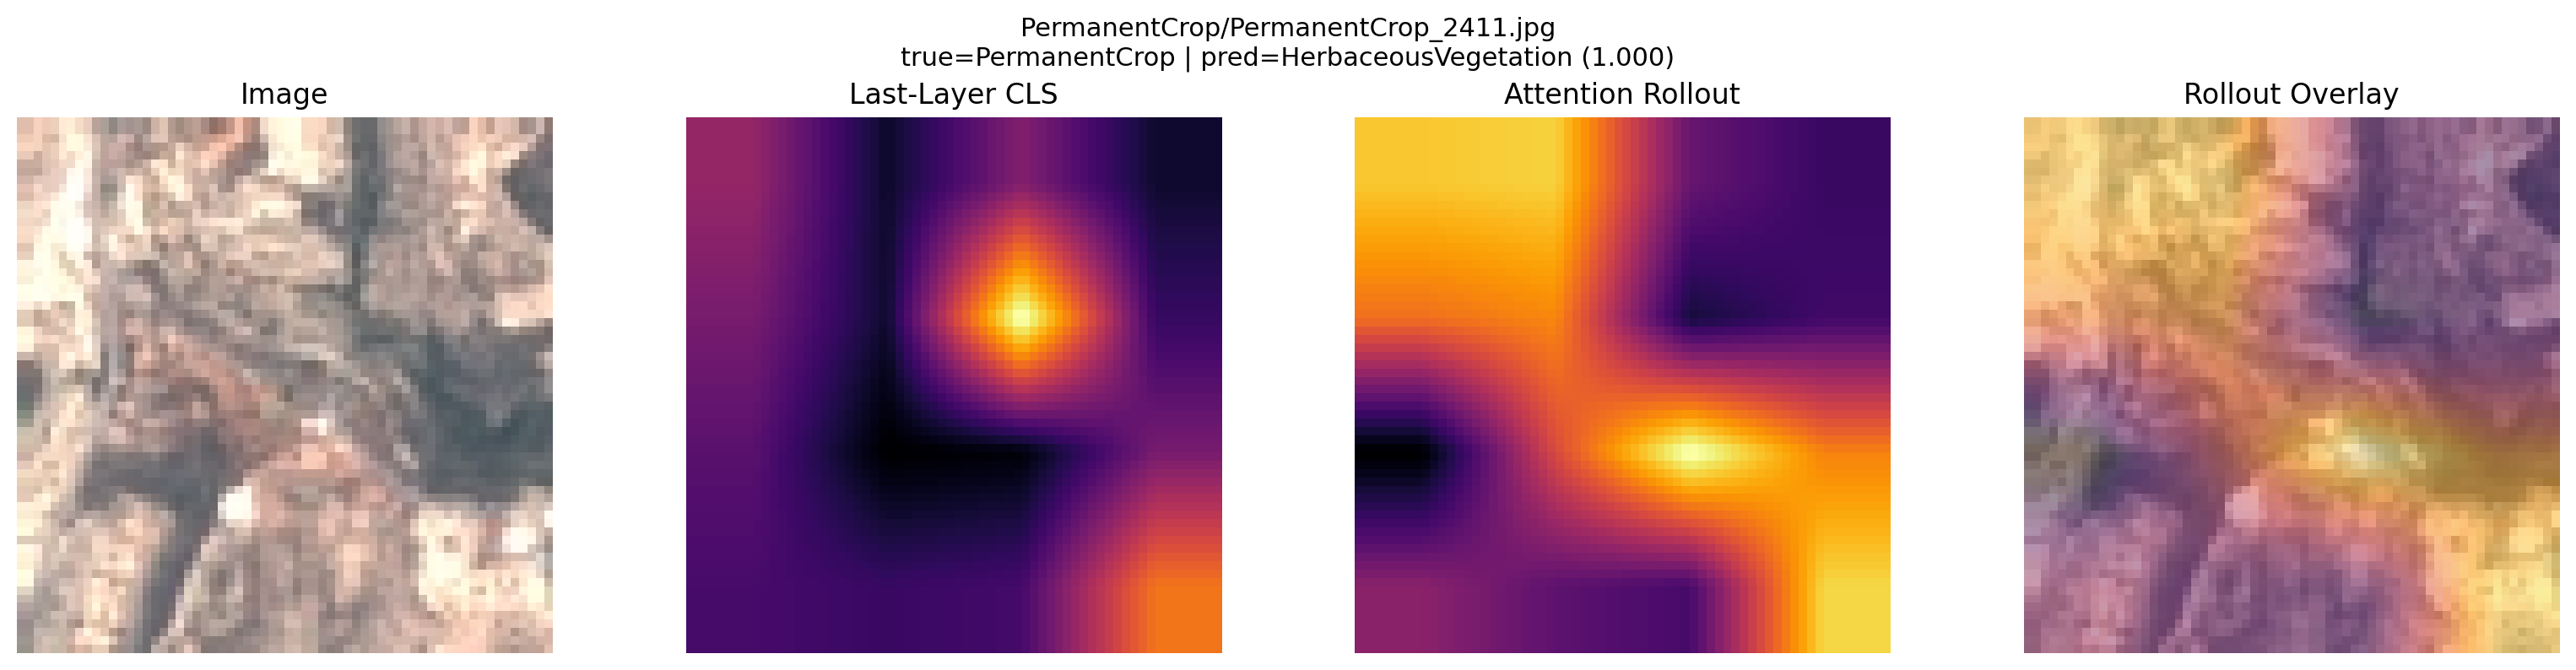
\includegraphics[width=\linewidth]{../outputs/vit_attention_batch/PermanentCrop_2411_incorrect_attention.png}
        \caption*{\footnotesize Incorrect: PermanentCrop \(\rightarrow\) HerbaceousVegetation (99.99\%)}
    \end{minipage}
    \hfill
    \begin{minipage}[t]{0.48\textwidth}
        \centering
        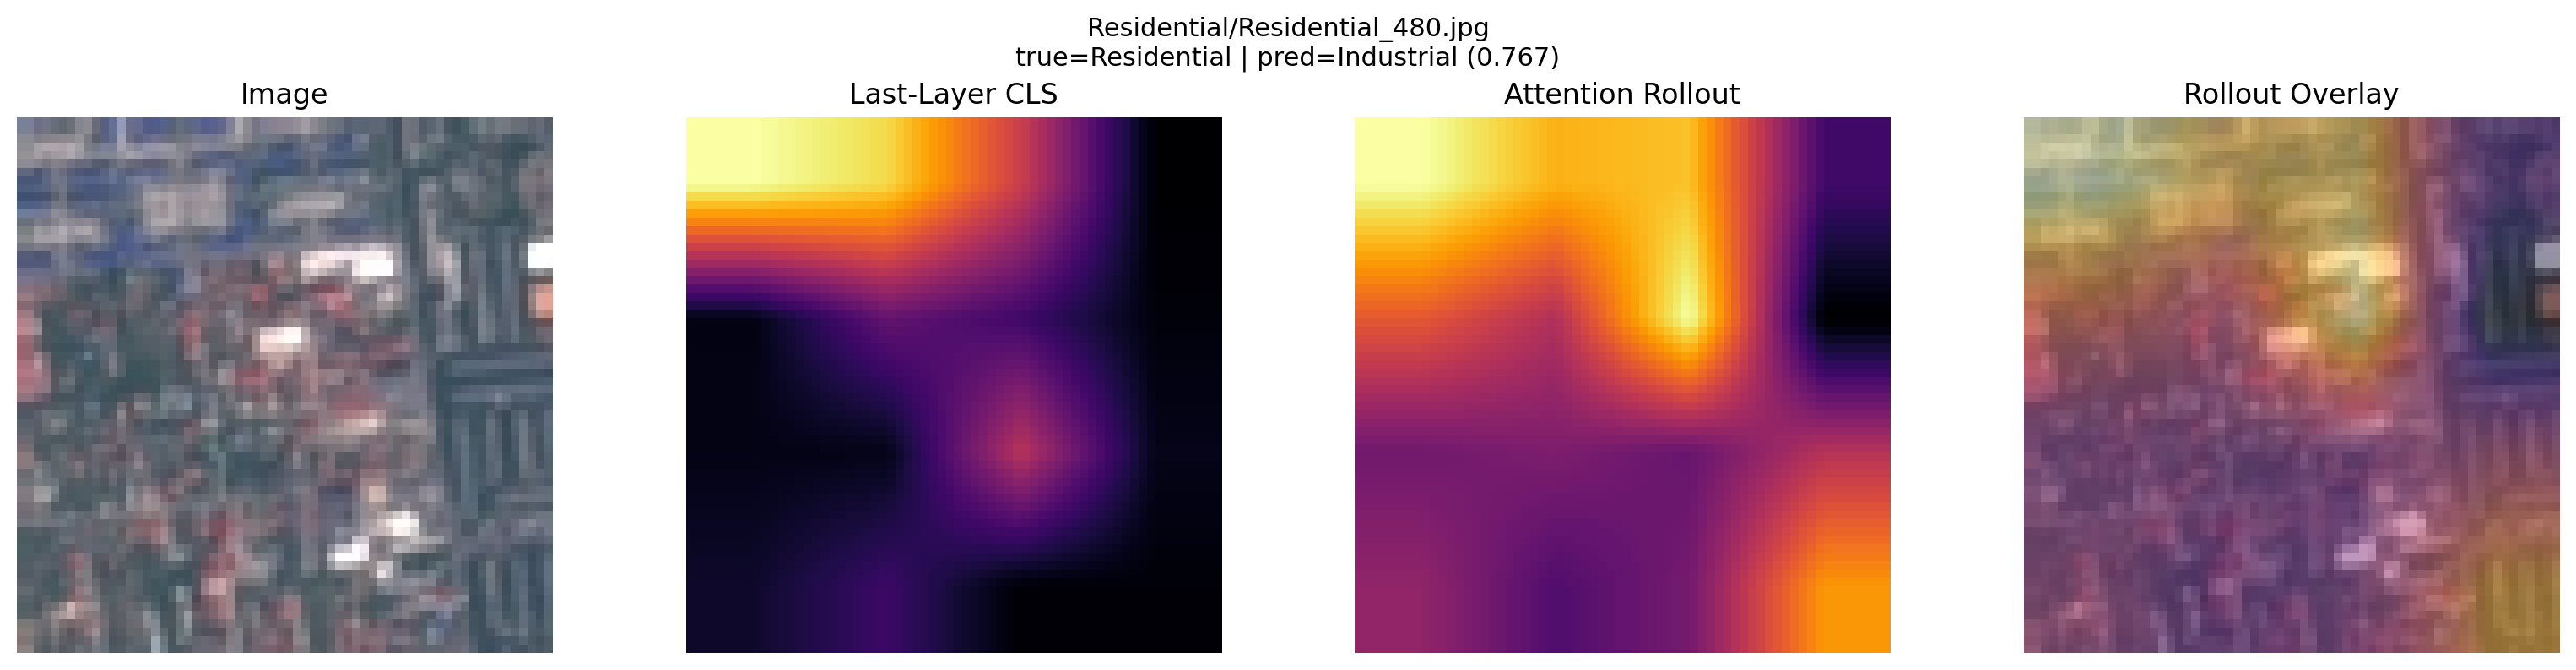
\includegraphics[width=\linewidth]{../outputs/vit_attention_batch/Residential_480_incorrect_attention.png}
        \caption*{\footnotesize Incorrect: Residential \(\rightarrow\) Industrial (76.74\%)}
    \end{minipage}
    \caption{Saved ViT-Small attention visualizations from the test set. The bottom row shows that the model can still produce confident but wrong predictions when classes share similar texture or spatial layout.}
    \label{fig:attention-montage}
\end{figure}

The attention montage makes two points clearer than the previous table-only summary. First, the correct examples show sharply localized focus on the dominant land-use pattern in the patch, which is consistent with the high-confidence predictions. Second, the incorrect cases illustrate why some EuroSAT classes remain difficult: PermanentCrop and HerbaceousVegetation share fine-grained vegetation texture, while Residential and Industrial can overlap in roof pattern and road layout. The repeated PermanentCrop \(\rightarrow\) HerbaceousVegetation confusion appears both here and in the full confusion matrices, so it is a dataset-level ambiguity rather than a one-off error.

\chapter{Conclusion}
This project produced a complete comparison of six EuroSAT RGB classifiers under a fixed and reproducible training pipeline. The main conclusion is that transfer learning mattered more than architecture choice or raw parameter count. All three pretrained models reached at least \(98.4\%\) test accuracy, while their from-scratch counterparts lagged behind by \(2.67\) to \(8.15\) percentage points.

Among the tested configurations, \BestModel{} was the strongest final model at \BestAcc{}\% test accuracy and \BestMacroFOne{}\% macro F1. The pretrained ViT-Small was nearly as strong, which shows that transformer-based models can perform very well on EuroSAT once pretrained weights are available. However, the from-scratch ViT-Small result also shows that the transformer is the least data-efficient option in this specific setup.

The experimental evidence therefore supports a practical recommendation: for a small-to-medium remote-sensing dataset, a pretrained CNN is the safest first choice, and a pretrained ViT becomes attractive when interpretability or architecture diversity is important. Essentially, a useful rule of thumb from these experiments is that, in low-data settings, the inductive bias of a CNN can outweigh the global modeling flexibility of a transformer. Future work could extend this report with multispectral EuroSAT experiments, robustness tests, or a larger transformer family.

\begin{thebibliography}{9}
\addcontentsline{toc}{chapter}{References}

\bibitem{helber2019}
P. Helber, B. Bischke, A. Dengel, and D. Borth,
``EuroSAT: A Novel Dataset and Deep Learning Benchmark for Land Use and Land Cover Classification,''
\emph{IEEE Journal of Selected Topics in Applied Earth Observations and Remote Sensing}, vol. 12, no. 7, pp. 2217--2226, 2019.

\bibitem{he2016}
K. He, X. Zhang, S. Ren, and J. Sun,
``Deep Residual Learning for Image Recognition,''
in \emph{Proceedings of the IEEE Conference on Computer Vision and Pattern Recognition}, 2016, pp. 770--778.

\bibitem{simonyan2015}
K. Simonyan and A. Zisserman,
``Very Deep Convolutional Networks for Large-Scale Image Recognition,''
in \emph{International Conference on Learning Representations}, 2015.

\bibitem{huang2017}
G. Huang, Z. Liu, L. van der Maaten, and K. Q. Weinberger,
``Densely Connected Convolutional Networks,''
in \emph{Proceedings of the IEEE Conference on Computer Vision and Pattern Recognition}, 2017, pp. 4700--4708.

\bibitem{vaswani2017}
A. Vaswani et al.,
``Attention Is All You Need,''
in \emph{Advances in Neural Information Processing Systems}, 2017, pp. 5998--6008.

\bibitem{dosovitskiy2021}
A. Dosovitskiy et al.,
``An Image Is Worth 16x16 Words: Transformers for Image Recognition at Scale,''
in \emph{International Conference on Learning Representations}, 2021.

\bibitem{deng2009}
J. Deng, W. Dong, R. Socher, L.-J. Li, K. Li, and L. Fei-Fei,
``ImageNet: A Large-Scale Hierarchical Image Database,''
in \emph{Proceedings of the IEEE Conference on Computer Vision and Pattern Recognition}, 2009, pp. 248--255.

\bibitem{pan2010}
S. J. Pan and Q. Yang,
``A Survey on Transfer Learning,''
\emph{IEEE Transactions on Knowledge and Data Engineering}, vol. 22, no. 10, pp. 1345--1359, 2010.

\bibitem{loshchilov2019}
I. Loshchilov and F. Hutter,
``Decoupled Weight Decay Regularization,''
in \emph{International Conference on Learning Representations}, 2019.

\end{thebibliography}

\end{document}
